\begin{figure*}[!t]
    \centering
    \subfloat[Accuracy Comparison]{
        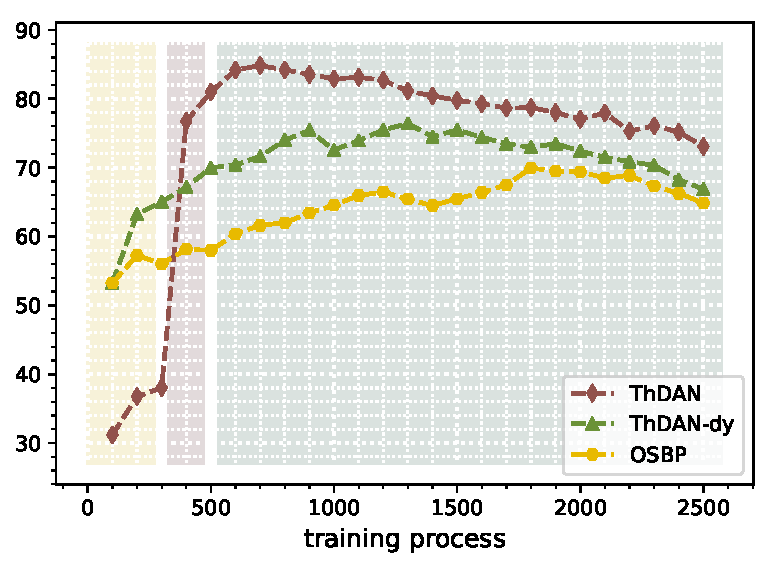
\includegraphics[width=0.33\textwidth]{contents/figures/pdf/analysis/Compare.pdf} 
        \label{figure: compares}
    } 
    \subfloat[OS and OS* Comparison]{
        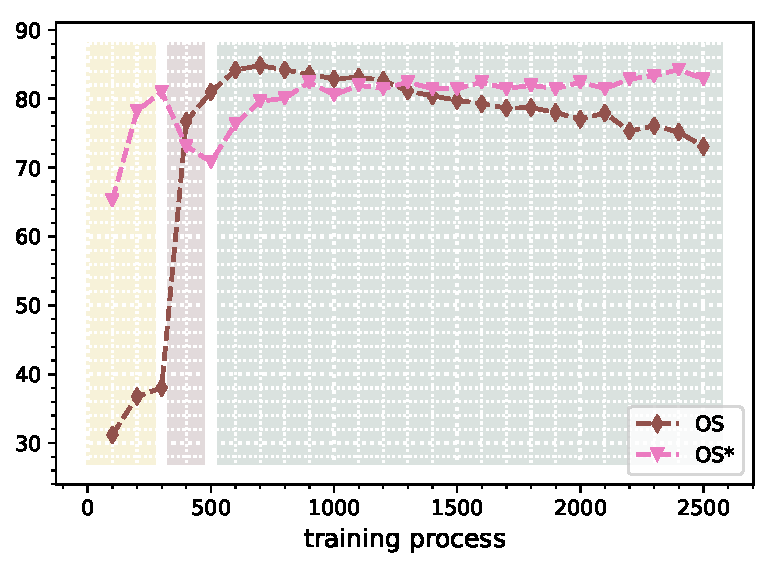
\includegraphics[width=0.33\textwidth]{contents/figures/pdf/analysis/OS.pdf} 
        \label{figure: OS and OS*}
    }
    \subfloat[Selection Accuracy]{
        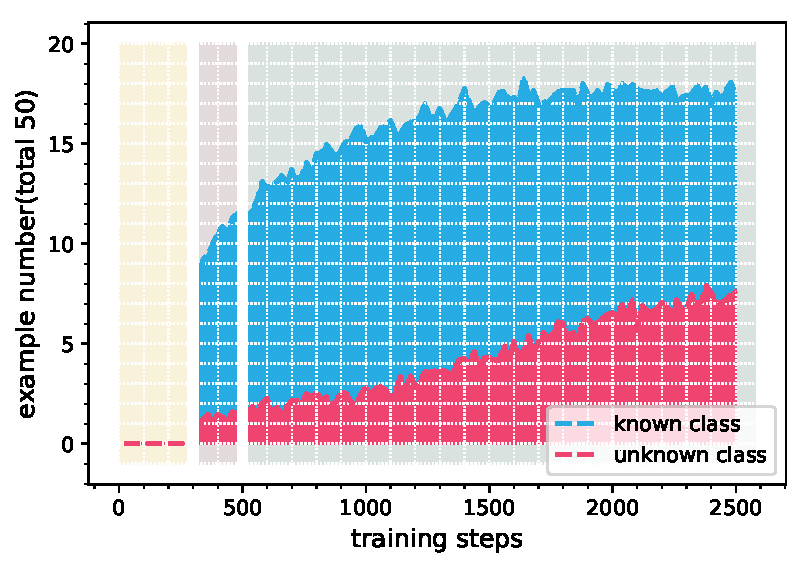
\includegraphics[width=0.33\textwidth]{contents/figures/pdf/analysis/Selection.pdf} 
        \label{figure: example selection record}
    }
    \\
    \hspace{0mm}
    \subfloat{
        
\includegraphics[width=0.32\textwidth]{contents/figures/pdf/analysis/annotation.pdf}
        } 
    \caption{
        Empirical analysis of ThDAN, we use three different color to denote different training stage as \figurename{\ref{figure: offset changing}} dose.
        (\textbf{a}): The comparison of accuracy between our model and OSBP. 
        (\textbf{b}): The \textit{All Class Accuracy \textbf{OS}} and \textit{Known Class Accuracy \textbf{OS*}}  of ThDAN during training.
        (\textbf{c}): The number of correctly selection and false selection during training. 
    }
    \label{figure: analysis}
\end{figure*}